\chapter{Firebase}                %crea il capitolo
%%%%%%%%%%%%%%%%%%%%%%%%%%%%%%%%%%%%%%%%%imposta l'intestazione di pagina
\lhead[\fancyplain{}{\bfseries\thepage}]{\fancyplain{}{\bfseries\rightmark}}
\section{Storia}                 %crea la sezione


Firebase è una piattaforma Mobile backend as a service (MBaaS) che consente
di interfacciare applicazioni mobili e web app ad un cloud backend, fornendo allo sviluppatore servizi utili per la gestione degli utenti, storage, notifiche push ed altri strumenti di analisi e sviluppo.\\
Il modello su cui si basa la piattaforma è relativamente recente poichè appoggiandosi al cloud computing, fornisce uno servizio globale e uniforme per connettere client differenti offrendo una sincronizzazione dei dati in tempo reale.\\
Lo sviluppo di Firebase iniziò dall'omonima azienda che nel 2011 sviluppò la piattaforma con l'idea di fornire un servizio in grado di sincronizzare dati in tempo reale, successivamente ricevette grande interessa da parte di Google che nel 2014 acquistò\footnote{https://techcrunch.com/2014/10/21/google-acquires-firebase-to-help-developers-build-better-realtime-apps/} Firebase e altre startup simili, integrandole con i suoi servizi Google Cloud Platform.


%https://gigaom.com/2013/06/20/firebase-gets-5-6m-to-launch-its-paid-product-and-fire-up-its-base/
% \begin{figure}[!hb]
%   \centering
%   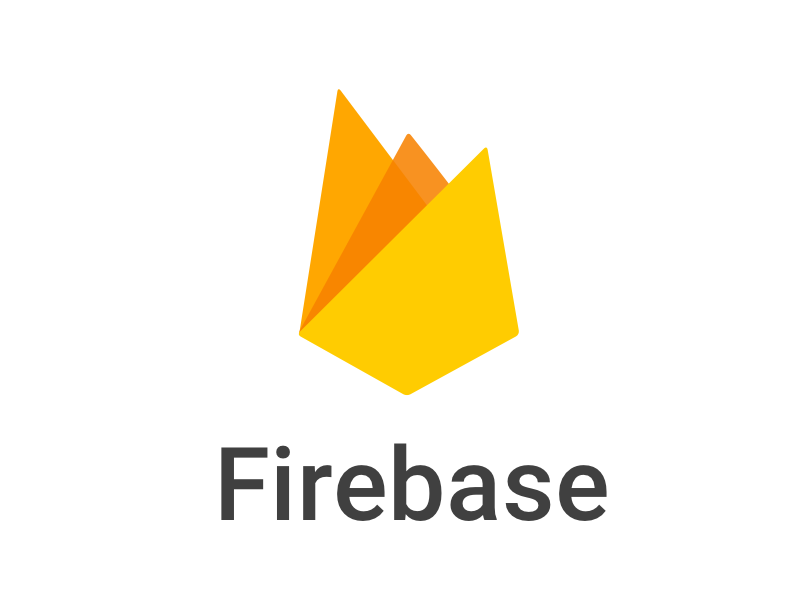
\includegraphics[width=0.25\textwidth]{immagini/firebase.png}
%   \caption{Firebase logo.}
%   \label{fig:firebase logo}
% \end{figure}




\section{Servizi}                 %crea la sezione
Firebase offre diversi servizi, mettendo a disposizione anche SDK (Software Development Kit) e API (Application Programming Interface) multipiattaforma (Android, Ios, JavaScript, C++, Unity) per interagire con essi.\\
I servizi\footnote{https://firebase.google.com/products/} offerti da Firebase sono circa 20, realizzati per facilitare lo sviluppo e la gestione del backend, permettendo ad uno sviluppatore di concentrarsi maggiormente sulla parte client e meno sulla manutenzione e gestione del backend.\\
Tra i vari servizi forniti, quelli più utili, nell'ambito dello sviluppo software sono:


\begin{itemize}                         %crea un elenco puntato
\item \textbf{Firebase Cloud Messaging}: Soluzione cross-platform per la gestione di notifiche push su Android iOS e Web.

\item \textbf{Firebase Auth}: Servizio per la gestione degli utenti con il supporto del social login per Facebook, Github, Twitter, Google.

\item \textbf{Realtime Database}: Database NoSQL con il supporto della sincronizzazione in tempo reale dei dati fra diversi client.

\item \textbf{Firebase Storage}: Servizio che offre il trasferimento e l'hosting sicuro dei file.

\item \textbf{Firebase Hosting}: Web hosting che fornisce file utilizzando CDN (Content Delivery Network) e HTTP Secure (HTTPS).

\item \textbf{Cloud Functions}: Servizio che permette di eseguire script JavaScript ogni volta che vi è un cambiamento nel database.

\item \textbf{Firestore Database}: Database NoSQL basato su documenti con il supporto della sincronizzazione in tempo reale.
\end{itemize}




\section{Database}                 %crea la sezione
Google offre due differenti database con supporto della sincronizzazione dei dati in tempo reale:

\begin{itemize}
  \item \textbf{RealTime Database}
  \item \textbf{Cloud Firestore}
\end{itemize}


\textbf{RealTime Database} è un cloud database NoSQL che memorizza i dati in un unico file JSON. Il database è organizzato attraverso un modello gerarchico ad albero con un unica radice ed ha una struttura senza schema che può cambiare nel tempo.\\
Utilizzando l'SDK, tutte le richieste effettuate al RealTime Database vengono memorizzate localmente nella cache del client e vengono aggiornate in tempo reale al susseguirsi di modifiche ed eventi all'interno del Database.\\
Quando il dispositivo precedentemente offline riacquista la connessione, l'SDK del Realtime Database sincronizza le modifiche dei dati locali con gli aggiornamenti remoti che si sono verificati mentre il client era offline, risolvendo automaticamente eventuali conflitti.\\


\textbf{Cloud Firestore} è un cloud database NoSQL basato sulla memorizzazione dei dati sotto forma di documenti e collezioni, anche la sua struttura è senza schema e può quindi cambiare nel tempo.\\
Il modello di memorizzazione dei dati è basato sui documenti che possono contenere  stringhe e numeri, date, oggetti complessi e annidati.\\
Questi documenti sono archiviati in raccolte, chiamate collezioni che contengono i documenti, ma è anche possibile creare sub-collezioni all'interno dei documenti e creare strutture gerarchiche di dati che scalano man mano che il database cresce.\\
Gli unici limiti imposti da Firestore sono: la dimensione di un singolo documento che è di 1 MiB (1,048,576 bytes) e un massimo di 100 collezioni annidate.\\
L'SDK del database Firestore mantiene i dati aggiornati attraverso una buona gestione del caching, i client invece utilizzando appositi listener offrono una sincronizzazione dei dati in tempo reale.\\
L'aggiunta di listener oltre a informare il client su modifiche effettuate nel database, permette di memorizzare le richieste effettuate in precedenza e mantenere una copia delle risposte del server nella cache, offrendo quindi un supporto offline dei dati.

I tipi di dato messi a disposizione da Firestore sono:
\begin{table}[h]
\begin{center}
\begin{tabular}{|p{3cm}|p{10cm}|}
    \hline
\textbf{Tipo} & \textbf{Descrizione} \\ \hline
Array & non può contenere un altro valore array. \\ \hline
Boolean & falso, vero  \\ \hline
Date & Memorizzato in formato timestamp \\ \hline
Float & precisione numerica a 64 bit \\ \hline
Geo Point & Punto geografico contentente latitudine e longitudine \\ \hline
Integer & Intero Numerico a 64 bit \\ \hline
Map & Rappresenta un oggetto  \\ \hline
Null & valore nullo \\ \hline
Reference & Riferimento ad un'altro documento nel database  \\ \hline
String & Stringa di testo codificata in UTF-8.\\
\hline
\end{tabular}
\caption[Dati Firestore]{Tipi di dato Firestore}\label{tab:Firestore Tipi di dato}
\end{center}
\end{table}

L' interrogazione del database Firestore attraverso query risulta essere molto espressiva ed efficiente. La creazione delle query permette di filtrare i dati all'interno di un documento o filtrare collezioni, con la caratteristiche basilari delle interrogazioni: l'ordinamento, il filtraggio e limiti sui risultati di una query. Si possono filtrare anche sottocampi di un oggetto Map, ma non è possibile filtrare o ordinare un elemento di tipo ``Reference'' che serve solo ad indicare il riferimento di un documento all'interno del database.\\
Cloud Firestore offre un SDK con una buona integrazione per dispositivi mobili Android, iOS e web apps, ma permette l'utilizzo dei servizi anche offrendo SDK aggiuntive per altri linguaggi di programmazione come: NodeJS, Java, Python, e GO.\\
Ricapitolando, possiamo definire Firestore come una nuova versione di Firebase RealTime con una miglior struttura interna, una buona memorizzazione dei dati e una espressività delle query maggiore.

\begin{table}[h]
\begin{center}
\begin{tabular}{|p{7.5cm}|p{7cm}|}
    \hline
    \textbf{RealTime Firebase} & \textbf{Firestore} \\ \hline
    Memorizza i dati in un unico file JSON & Memorizza i dati in collezioni contententi documenti \\ \hline
    Supporto per i dati offline su Android e iOS & Supporto per i dati offline su Android, iOS e Web \\ \hline
    Depp Query con ordinamento e condizioni sui dati limitate & Query con ordinamento, condizioni sui dati, indicizzazione, alte performance \\ \hline
    Memorizzazione di dati come singole operazioni. & Memorizzazione e transizioni sui dati atomiche.\\ \hline
    Validazione dei dati manuale, e settaggio manuale di regole di protezione sui dati &  Validazione dei dati automatica, e regole di protezione sui dati manuali\\
\hline
\end{tabular}
\caption[Confronto tra Firebase e Firestore ]{Confronto dei due database Firebase}\label{tab:Confronto tra  Firestore e Firebase}
\end{center}
\end{table}


\subsection{Database Rules}                 %crea la sezione
Firebase offre per i suoi due database la possibilità di inserire delle restrizioni e regole di sicurezza per l'accesso al Database, chiamate Database Rules. Le Database Rules determinano chi ha accesso in lettura e scrittura al database o a collezioni di dati all'interno del database, queste regole sono gestite utilizzando il pannello di controllo di Firebase, una volta scritte le regole queste vengono applicate automaticamente ad ogni modifica. Ogni richiesta di lettura e scrittura di dati nel database sarà completata solo se le regole lo consentono.\\
Entrambi i database: Real time e Firestore supportano le Database Rules, le differenze fra i due servizi riguardano il metodo con cui vengono scritte le regole e il tipo di controlli che è possibile effettuare.\\
Firebase permette di scrivere le regole utilizzando un file in formato JSON dove vengono definite le regole in base alla collezione in cui si trovano i dati, alla validazione dei dati o in base all'utente registrato su Firebase Auth.\\
Le regole applicate al database RealTime hanno una sintassi simile a JavaScript e mettono a disposizione del programmatore quattro tipi di controlli:

\begin{table}[h]
\begin{center}
\begin{tabular}{|p{2cm}|p{12cm}|}
    \hline
    {\textbf{Tipo}} & {\textbf{Descrizione}} \\ \hline
    .read & Descrive se e quando i dati possono essere letti dagli utenti.\\ \hline
    .write & Descrive se e quando i dati possono essere scritti dagli utenti\\ \hline
     .validate & Definisce l'aspetto di un valore formattato correttamente, se ha attributi figli e il tipo di dato\\ \hline
    .indexOn & Specifica una collezione da indicizzare per supportare l'ordine e l' interrogazione\\ \hline
\end{tabular}
\caption[Firbase Rules ]{Firebase Database Rules}\label{tab:Firebase Database Rules}
\end{center}
\end{table}

Le regole per il database RealTime vengono memorizzate in formato JSON sui server Firebase, un esempio di alcune regole applicate è il seguente:

\begin{lstlisting}[language=javascript,caption={Firebase Rules esempio }]
{
  "rules": {
    "users": {
      "$uid": {
        ".write": "$uid === auth.uid"
      }
    },
    "collection2": {
     ".validate": "newData.isString() && newData.val().length < 100"
   }
  }
}
\end{lstlisting}


Le regole di sicurezza del database Firestore sono simili a quelle del RealTime Database ma prevedono un controllo degli accessi e della validazione dei dati in un formato più semplice ed espressivo.\\
Tutte le regole di sicurezza Firestore sono costituite da dichiarazioni di corrispondenza chiamate ``match'' che identificano i documenti nel database e consentono la creazione di espressioni che controllano l' accesso a tali documenti.\\
Oltre alle regole di scrittura, lettura, validazione è possibile creare funzioni ausiliarie per semplificare e rendere più intuitiva la scritture delle regole.\\
Un esempio di scrittura di alcune regole su un database Firestore è il seguente:

\begin{lstlisting}[language=javascript,caption={Firestore Database Rules}]
service cloud.firestore {
  match /databases/{database}/documents {
    function signedInOrPublic() {
      return request.auth.uid != null || resource.data.visibility == 'public';
   }
  match /cities/{city} {
      allow read: if request.auth.uid != null;
      allow create: if exists(/databases/$(database)/documents/users/$(request.auth.uid))
  }
 }
}
\end{lstlisting}



\section{Cloud Functions}                 %crea la sezione

Le Cloud Functions consentono di eseguire script backend in risposta a modifiche effettuate nel database Firestore o RealTime, o sullo storage Firebase. I linguaggi utilizzati per scrivere le Cloud Functions sono JavaScript e TypeScript, una volta scritta una funzione essa viene memorizzata e gestita dai server Firebase e man mano che il carico aumenta o diminuisce, Google scala automaticamente il numero di istanze di server virtuali necessari per eseguire le funzioni.


Il ciclo di vita di una funzione è il seguente:
\begin{itemize}
  \item Lo sviluppatore scrive il codice per una nuova funzione, selezionando un provider di eventi (Realtime Database, Firestore, Storage) e definisce le condizioni in cui la funzione deve essere eseguita.
  \item Lo sviluppatore tramite un tool a linea di comanda invia la funzione sui server di Firebase.
  \item Quando il provider dell'evento genera un evento che corrisponde alle condizioni della funzione, il codice della funzione viene eseguito.
  \item Se sono presenti più eventi da gestire contemporaneamente, Google creerà più instanze per gestire il lavoro più velocemente.
  \item Quando lo sviluppatore aggiorna la funzione distribuendo il codice aggiornato, tutte le istanze per la vecchia versione vengono cancellate e sostituite da nuove istanze.
  \item Quando uno sviluppatore cancella una funzione, tutte le istanze vengono cancellate e la connessione tra la funzione e il provider dell' evento viene rimossa.
\end{itemize}


           % ends first column but not page
Cloud Functions mette a disposizione quattro tipi di controllo sul database:

\begin{table}[h!]
\begin{tabular}{|p{2cm}|p{12cm}|}
    \hline
    \textbf{Evento} & \textbf{Trigger} \\ \hline
    onCreate & Attivato quando si scrive un documento per la prima volta.\\ \hline
    onUpdate & Attivato quando esiste già un documento e se ne modifica un valore.\\ \hline
    onDelete & Attivato quando un documento con dati viene eliminato.\\ \hline
    onWrite & Attivato quando si attiva onCreate, onUpdate o onDelete.\\ \hline

\end{tabular}
\caption[Firestore Rules]{Controlli Cloud Functions}\label{tab:Controlli Cloud Functions}
\end{table}

La stesura di una funzione viene effettuata definendo funzioni JavaScript o TypeScript ed indicando il documento o la collezione sui cui si vuole fare riferimento, seguito dal tipo di evento:


\begin{lstlisting}[language=javascript,caption={Cloud functions esempio 1 }]
exports.myFunctionName = functions.firestore.document('users/koci').onWrite((event) => {
    ...
  });
exports.modifyUser = functions.firestore.document('users/{userID}').onWrite(event => {
    //  documento sottoforma di oggetto
    var document = event.data.data();
    // documento precedente alla modificarlo
    var oldDocument = event.data.previous.data();
    ...
});
\end{lstlisting}


\newpage              % ends first column but not page
\subsection{Esempi di utilizzo}
Le cloud functions possono essere utilizzate anche interagendo con gli altri servizi Firebase, un esempio di integrazione tipico potrebbe essere quello di creare l'anteprima di un immagine e salvarla su Firebase Storage:

\begin{figure}[!h]
  \centering
  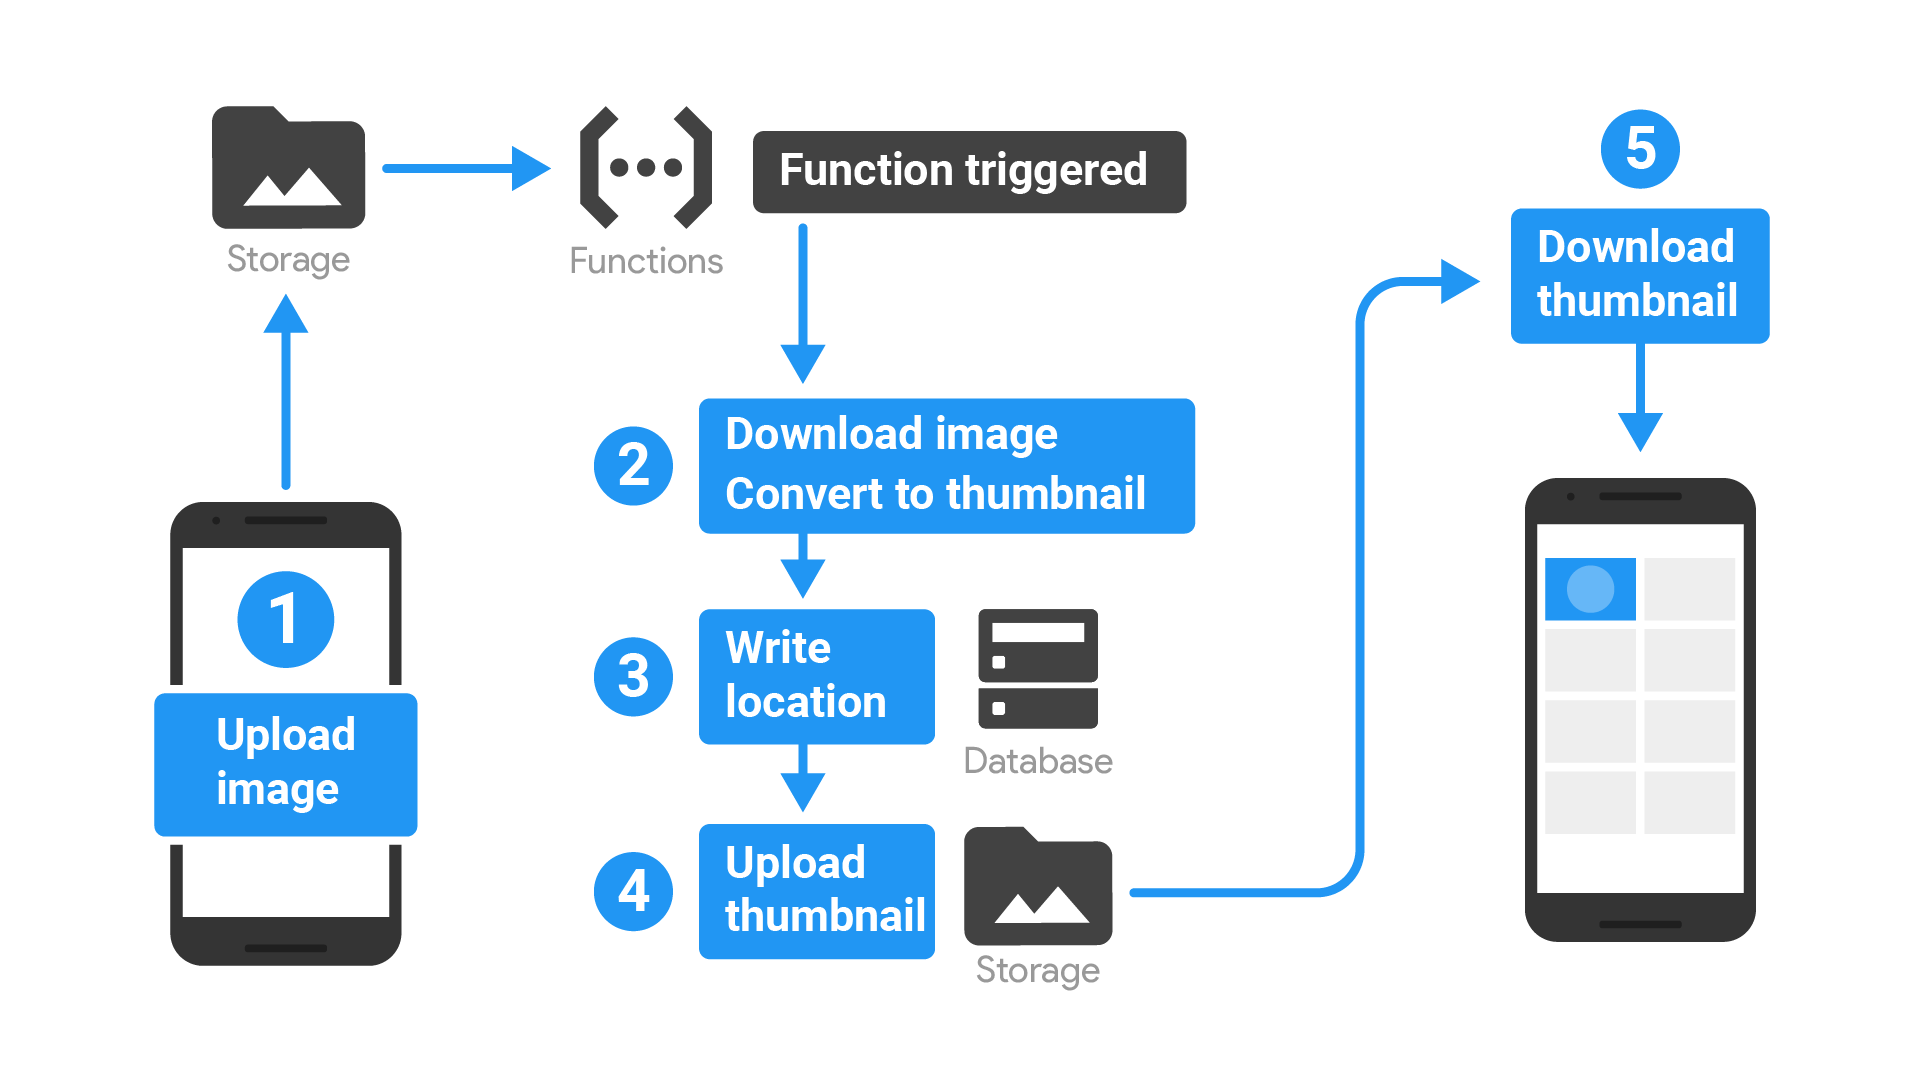
\includegraphics[width=0.5\textwidth]{immagini/functions_ex1.png}
  \caption{Firebase Storage e Cloud Functions esempio 1}\label{fig:Firebase Storage e Cloud Functions esempio 1}
\end{figure}

In questo esempio, una funzione del servizio Cloud Function rimane in ascolto su cambiamenti nello Storage in atttesa che un'immagine venga caricata, Quando un utente aggiungerà un immagine nello storage, verrà richiamata la funzione che scaricherà l'immagine e ne creerà una versione miniaturizzata, in seguito scriverà il riferimento della miniatura sul database, in modo che un'applicazione client possa trovarla e utilizzarla.
Un'altro esempio è l'utilizzo delle cloud functions per effettuare controlli su un tipo di linguaggio inappropriato all'interno di una chat,forum o commento:
la funzione esamina il testo, rimuove il linguaggio volgare e restituisce il testo revisionato.


\begin{figure}[!h]
\centering
  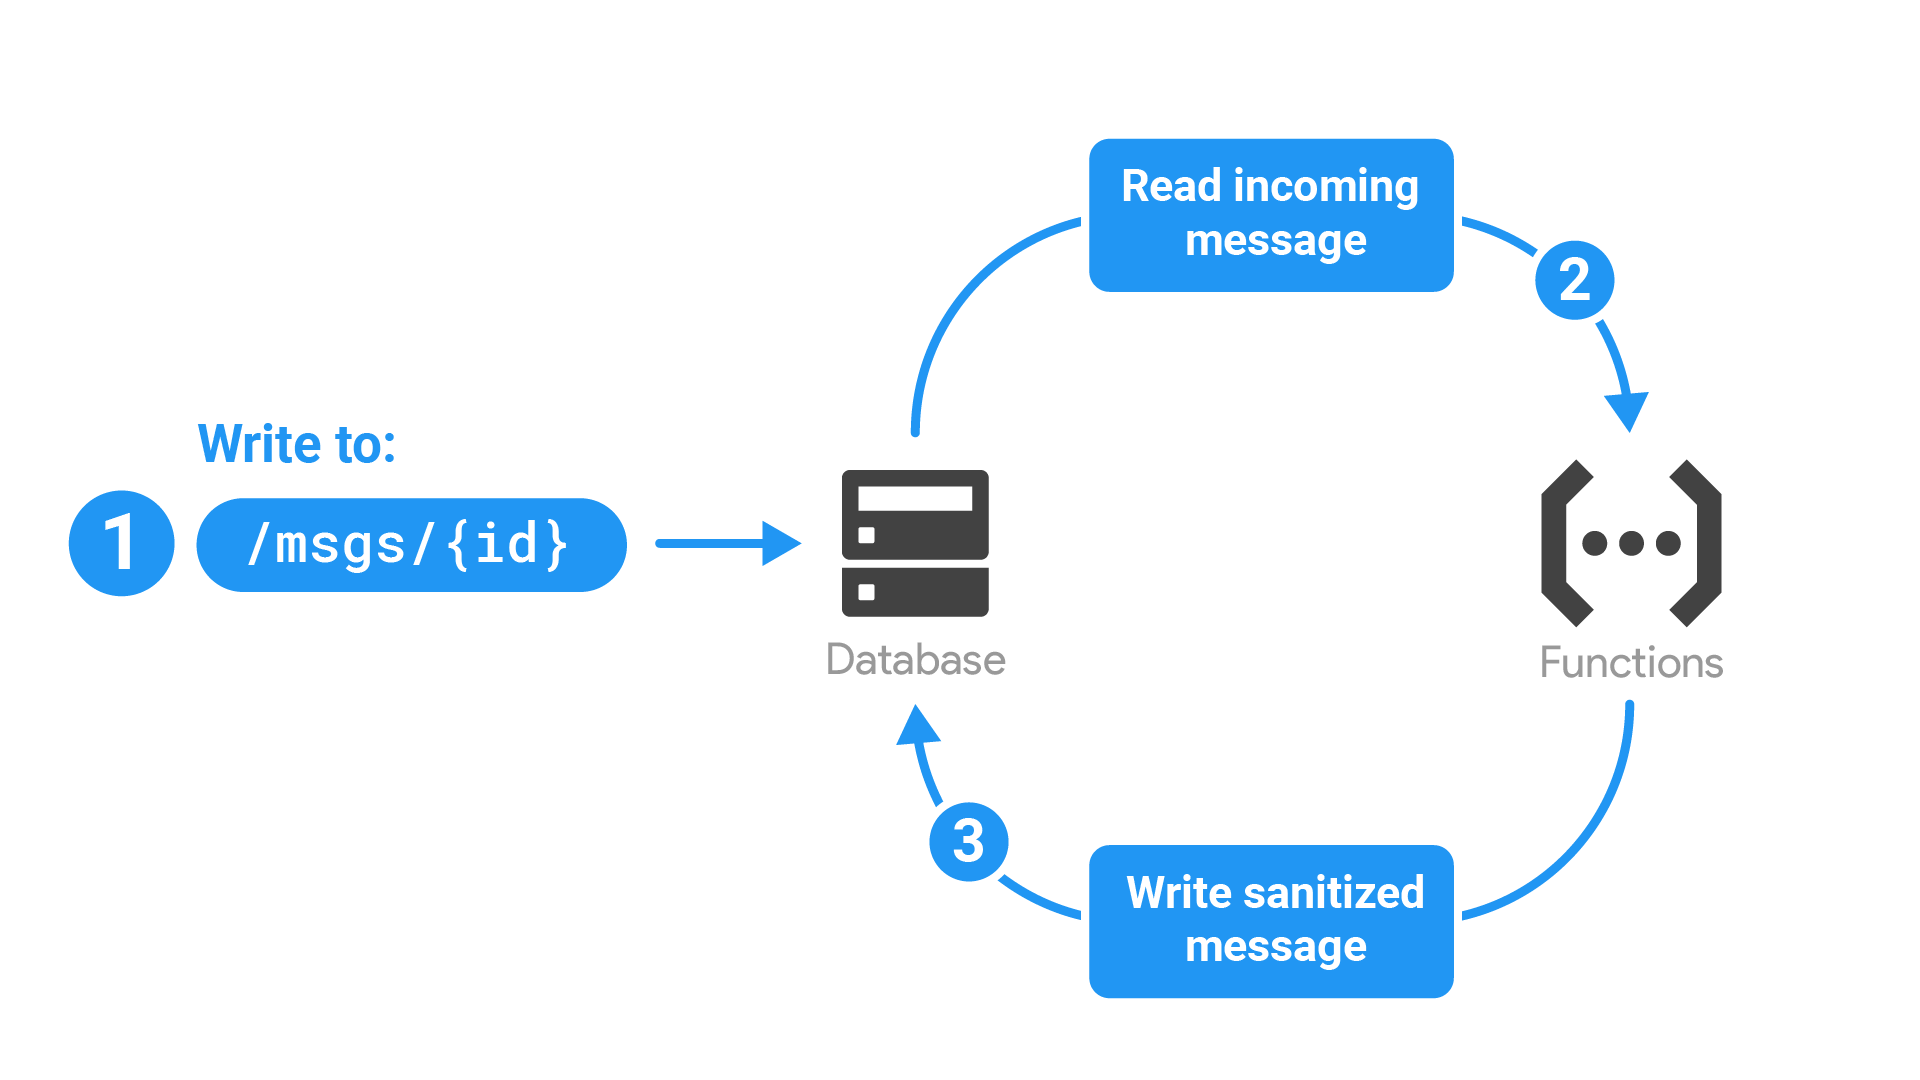
\includegraphics[width=0.5\textwidth]{immagini/functions_ex2.png}
  \caption{Firebase Storage e Cloud Functions esempio 2}
  \label{fig:Firebase Storage e Cloud Functions esempio 2}
\end{figure}


\newpage
%https://developer.xamarin.com/guides/android/data-and-cloud-services/google-messaging/firebase-cloud-messaging/
\section{Cloud Messaging}                 %crea la sezione
Firebase Cloud Messaging (FCM) è una soluzione di messaggistica multipiattaforma che consente di inviare messaggi tra dispositivi con la possibiltà, di notificare a una o più applicazioni client che sono disponibili nuovi dati.\\
è possibile inviare messaggi tramite l'Admin SDK\footnote{https://firebase.google.com/docs/admin/setup} o le API HTTP e XMPP, rispettando la dimensione massima di un messaggio corrispondente a 4KB.\\
I messaggi possono essere di due tipologie: messaggi di notifica e messaggi di dati, la differenza fra i due tipi di messaggi è il loro contenuto: i messaggi di notifica contengono un insieme predefinito di chiavi visualizzabili dall'utente, mentre i messaggi di dati contengono solo un insieme di chiave-valore definito da chi invia il messaggio.\\
Entrambi i messaggi richiedono di definire il campo obbligatorio ``token'' che è il riferimento ad un dispositivo o di un gruppo di dispositivi, questo token è generato tramite l'SDK di Firebase e deve essere memorizzato su un server per poter essere riutilizzato, in caso contrario l'SDK consente di aggiornare il token del dispositivo.

\begin{figure}[!hb]
  \centering
  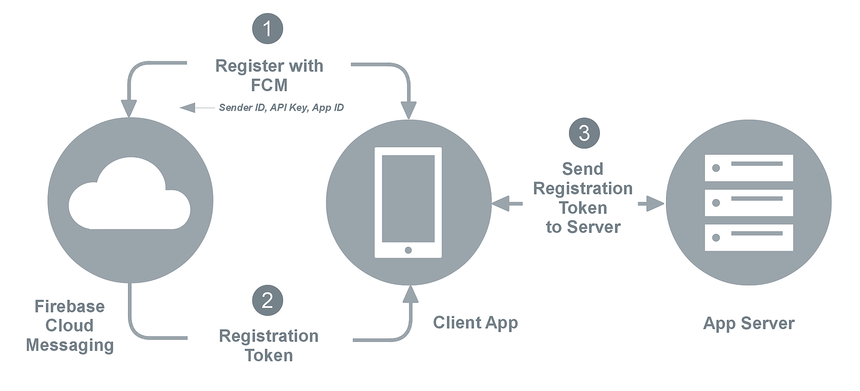
\includegraphics[width=1\textwidth]{immagini/fcm_token.png}
  \caption{Processo di generazione di un token per il servizio FCM.}
  \label{fig:Processo di generazione di un token per il servizio FCM}
\end{figure}

\newpage
La ricezione dei messaggi di Cloud Messaging è possibile solo se si utilizza l'apposito SDK e si ottiene un token, necessario per inviare un messaggio ad un dispositivo specifico.\\
All'avvio iniziale dell'applicazione, l'SDK FCM genera un token di registrazione per l'istanza dell'applicazione client.\\
I token e la ricezione dei messaggi possono essere controllati utilizzando le funzioni offerte dall'SDK.
La classe ``FirebaseInstanceIdService'' viene utilizzata per la gestione dei token, mentre la classe ``FirebaseMessagingService'' viene utilizzata per la gestione dei messaggi ricevuti.\\
Il token di registrazione può cambiare quando l'applicazione elimina il token, ripristina, reinstalla, disnistalla l'app, o quando vengono eliminate le cache e i dati dal dispositivo.


\subsection{Messaggi}
I messaggi di dati inviabili tramite l'SDK o richieste HTTPS possono essere di due tipi:
\begin{itemize}
    \item \textbf{Downstream Messaging}
    \item \textbf{Upstream Messaging}
\end{itemize}

I messaggi Downstream, permettono di inviare una notifica push dal Server verso il Client

\begin{figure}[!hb]
  \centering
  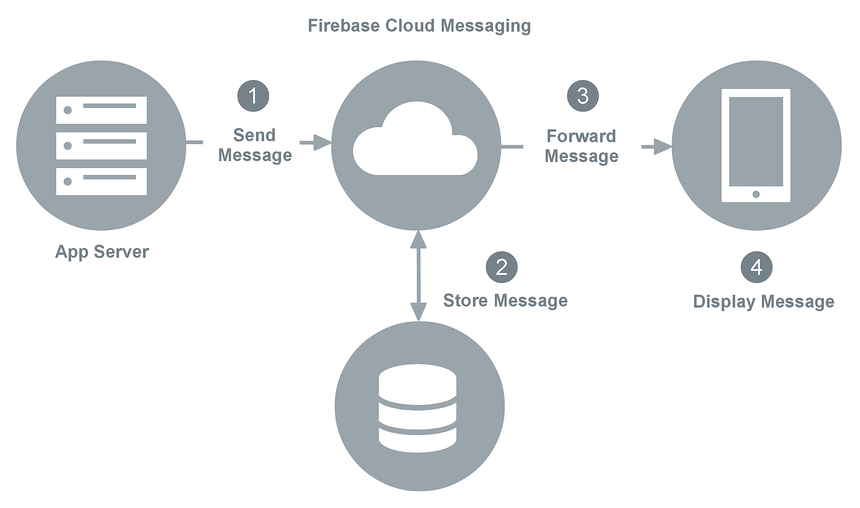
\includegraphics[width=0.55\textwidth]{immagini/fcm_down.png}
  \caption{Esempio downstream messaging - Firebase Cloud Messaging}
  \label{fig:Esempio downstream messaging - Firebase Cloud Messaging}
\end{figure}


\begin{itemize}
    \item Il server (per esempio Cloud Functions) invia il messaggio a FCM.
    \item Se il client non è disponibile, il server FCM memorizza il messaggio in una coda per la successiva trasmissione. I messaggi vengono conservati nella memoria FCM per un massimo di 4 settimane.
    \item Quando il dispositivo client è disponibile, FCM inoltra il messaggio all'applicazione.
    \item L'applicazione client riceve il messaggio da FCM, lo elabora e lo visualizza all'utente.
\end{itemize}

In alternativa oltre all'invio di un messaggio ad un singolo dispositivo FCM consente la creazione di gruppi di utenti, permettendo con un singolo token di inviare un messaggio a tutti i dispositivi appartenenti ad un gruppo.\\
Il funzionamento dei messaggi Upstream invece è analogo e permette di inviare messaggi da un dispositivo client ad un server (ad esempio Cloud Functions).\\
Sulla base del modello di pubblicazione/iscrizione invece, FCM consente anche di inviare un messaggio a più dispositivi che si sono registrati ad un particolare argomento.

\begin{figure}[!hb]
  \centering
  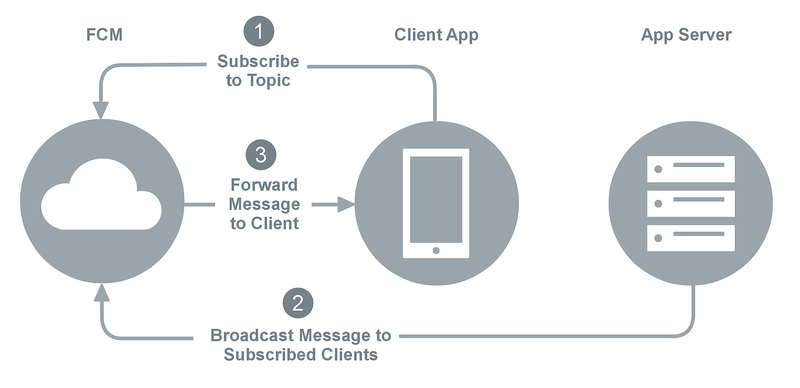
\includegraphics[width=0.8\textwidth]{immagini/fcm_topic.png}
  \caption{Esempio topic messaging - Firebase Cloud Messaging}\label{fig:Esempio topic messaging - Firebase Cloud Messaging}
\end{figure}

    \begin{itemize}
        \item L'applicazione client si iscrive ad un argomento inviando un messaggio di sottoscrizione al server FCM.
        \item Il server invia messaggi tematici a FCM per la distribuzione.
        \item FCM inoltra messaggi tematici ai client che si sono registrati a tale argomento.
    \end{itemize}

Per iscriversi a un argomento, l'applicazione client chiama la seguente funzione:

\begin{lstlisting}[language=java,caption={FCM topic}]
 FirebaseMessaging.getInstance().subscribeToTopic("news");
\end{lstlisting}

Per annullare l'iscrizione, l'applicazione client deve richiamare ``unsubscribeFromTopic()'' con il nome del topic dal quale disiscriversi.

\subsection{Parametri Cloud Messaging}
Oltre al destinatario è possibile definire anche la priorità di un messaggio, la durata, il suono, l'icona, il tempo di vita e altri parametri opzionali.\\
I principali parametri messi a disposizione da Firebase sono:

\begin{table}[!h]
\begin{center}
\begin{tabular}{|l|p{11cm}|}
\hline
\textbf{Paramentro} & \textbf{Descrizione} \\ \hline
Title &	Titolo della notifica \\   \hline
Body &	Testo della notifica \\   \hline
Sound  &	Suono da riprodurre quando il dispositivo riceve la notifica \\   \hline
Sottotitolo  &	Sottotitolo della notifica \\   \hline
Icon & Icona della notifica \\   \hline
Timetolive & Specifica per quanto tempo (in secondi) il messaggio deve essere conservato se il dispositivo è offline  \\   \hline
Clickaction & L'azione associata al click della notifica \\   \hline

\end{tabular}
\caption[Cloud Messaging paramentri]{Cloud Messaging parametri}\label{tab:Cloud Messaging parametri}
\end{center}
\end{table}

\newpage
\subsection{Priorità}
Esistono due opzioni per assegnare la priorità di consegna ai messaggi: normale ed alta priorità. Il recapito di messaggi normali e di alta priorità funziona in questo modo:
\begin{itemize}
\item  \textbf{Priorità normale}: I messaggi vengono inviati immediatamente quando l'app è in primo piano, quando invece il dispositivo è in modalità Doze o l'applicazione è in standby la consegna potrebbe essere ritardata per risparmiare la batteria, i messaggi in questo caso richiedono di pianificare un Job FJD (Firebase Job Dispache) o un JobIntentService per gestire la notifica quando il dispositivo sarà nuovamente online.
\item \textbf{Alta priorità}: Il server Cloud Messaging tenta di inviare immediatamente il messaggio ad alta priorità, consentendo al servizio, attraverso l'SDK di cambiare lo stato del dispositivo e di eseguire alcune elaborazioni limitate (compreso un accesso alla rete molto limitato).
\end{itemize}





\section{FirebaseUI}                 %crea la sezione
FirebaseUI è un insieme di librerie open-source\footnote{https://firebaseopensource.com/projects/firebase/firebaseui-android/} disponibile per diverse piattaforme, che consentono di semplificare lo sviluppo di un applicazione che utilizza Firebase.\\
La libreria offre una versione semplificata per gestione dell'autenticazione, fornendo metodi che si integrano con i più comuni social, migliorando la comunicazione tra le View dell'interfaccia utente e il database, e facilita inoltre il collegamento e le richieste con il servizio Firebase Storage.\\
FirebaseUI dispone di moduli separati per utilizzare le varia librerie dedicate ai servizi:
\begin{itemize}
  \item  FirebaseUI Auth
  \item  FirebaseUI Firestore
  \item  FirebaseUI Database
  \item  FirebaseUI Storage
\end{itemize}


FirebaseUI-Auth cerca di gestire tutte le possibili casistiche che si possono riscontrare durante il login e la registrazione di un nuovo utente.
La libreria FirebaseUI-Auth offre una integrazione con i social login più diffusi (Google, Facebook, Twitter) e una buona integrazione con Smart Lock per memorizzare e recuperare le credenziali, consentendo l' accesso automatico e il single-tap sign-in, gestendo anche casi d'uso più complessi come il recupero dell'account e il collegamento di account multipli che sono sensibili alla sicurezza e difficili da implementare correttamente utilizzando le API di base fornite da Firebase.\\
FirebaseUI-Firestore semplifica la comunicazione e l'interazione dei dati fra Cloud Firestore e l'interfaccia utente dell' applicazione, fornendo un adapter personalizzato (FirestoreRecyclerAdapter) che consente la manipolazione e la sincronizzazione automatica dei dati, senza dover scrivere codice ripetitivo per ogni adapter che si interfaccia con il database.
\clearpage{\pagestyle{empty}\cleardoublepage}
